\documentclass[a4paper]{report}
\title{Using fNIRS to Detect Mental Workload and Emotional Valence in web form filling task}%changing the layout of long web forms
\date{2015-09-18}
\author{Kristiyan Lukanov}
\usepackage{graphicx}
\usepackage{amsmath}
\usepackage{caption} 
\captionsetup[table]{skip=10pt}
\renewcommand{\bibname}{References}
\renewcommand{\arraystretch}{1.3}
\begin{document}
	\pagenumbering{gobble}
	\maketitle
	\newpage
	\pagenumbering{arabic}
	
	\section*{Acknowledgements}
	lorem ipsum 
	\newpage
	
	\section*{Abstract}
	In this dissertation we evaluated a desktop interface using functional near infrared spectroscopy(fNIRS), and verified the practicality of this brain imaging modality. More specifically, we tested the web page layout of online insurance claim process...
	\newpage
	\tableofcontents
	\newpage
	
	\chapter{Introduction}
	%The whole thesis should be third person past tense. Participants were asked to read and sign
	- Start with the problem
	
	Users often has to fill web pages containing more than 10 forms, like registering for a web site, posting classified ad, or sending online insurance claim. Sometimes this is really important, like filling insurance claim forms. People often dislike the fact that they should fill a long form and that makes the claim process difficult. That is why we are interested in measuring the mental workload in this type of tasks
	
	fNIRS has been suggested as a suitable for HCI studies, however when reviewing the literature review, according to our knowledge only one study was found\cite{peck2013using} that uses hemodynamic data from fNIRS to compare and evaluate different variations of an interface.
	
	we want to if new web form designs will make the task easier
	
	Importance of those forms(how they should be accurate and unaiding)
	 However this often encountered task in our daily lives is not well researched in the field of cognitive science.	
	
	 -it is important measure, especially for critical tasks such as, aircraft controller, where operator with workload overload could cause accidents and cost human lifes.
	
	With the advance of technology, brain imaging techniques have emerged, like MRI, EEG, and fNIRS which were initially, used for medical research and purposes. In recent years the popularity of these brain imaging techniques has risen in the HCI field because of their ability to image brain data.
	
	videos shown are aversive stimuly(ili otbluskva6ti stimuli, ne e sigurno da se proveri) . 
	
	The studies using brain imaging were limited because they were presenting emotional cues, but in this study we check whether we can elucidate laterized emotions giving subjected emotional cue-less web interface. hich will be very useful in HCI area
	\section{Purpose of study}
		 We aim to find the most efficient layout for entering information on an web interface that has more than 10 forms, as this process is often encountered during daily web surfing, for example, when user registers to a new web site, or enter information for financial institutions, like insurance companies and banks.
	\section{Research questions}
		Can we measure mental workload with fnirs?
		- Could we detect emotional valence with fnirs?
		- Which of the three layouts is has the least mental workload and users preference?
		- Could we detect emotional valence, from web interface that has no emotional cues. This can very useful in HCI evaluations.
	\section{Industry partner}
		This work has been motivated by the need of entity partner funding my masters course. The industry partner has a insurance CRM software, and the aim of the study is to provide insights in the web form filling process by testing the layout of the web pages.
		
	\section{Structure of the thesis}
		In the next chapter we will first review the background literature behind usability and web forms, mental workload and working memory, Brain sensing techniques, Emotion processing. In chapter 3 we will describe the User study section experiment done in the . And finally we will discuss the results from the experiment and propose a conclusion.
\chapter{Literature review}
	In the HCI field  evaluation approaches ca be divided in three general categories: analytical, field study and lab study\cite{rogers2007interaction}. First, analytical methods are designed to predict user behaviour such as, heuristic evaluation or expert reviews, so no experiment has to be conducted. Second, field studies are conducted in context in order to collect relevant and valid data, like observations. Lastly, lab studies use artificial settings but the experiment variables can be controlled easier, and also, comparative tests can be conducted. Our aim of the study is to evaluate a web form filling interface for the insurance domain, and more precisely, online auto insurance claim process. Therefore we are interested in conducting lab study because we cannot simulate road accident and we are able to compare variations of insurance claim web form. Furthermore, there are variety of evaluation methods, like interviews which will give us information about what users think about the interface, or observations which will let us recognize typical behaviour of users and obstacles they encounter while using the interface.\\
	
	It has to be mentioned that lab studies give us the chance to prepare the environment and record more performance measures which provide valuable objective information. Typical performance measures in usability experiments are time to complete, errors encountered, and number of events. In general, mental workload and emotional valence are of high interest in HCI evaluations because measuring workload gives us important information about the task demands and also, knowing whether a user is feeling positive or negative towards an interface or task may give us valuable information about their general preferences. Furthermore, Nielsen\cite{nielsen1994measuring} suggested that user preferences correlate with user performance, thus we can rely solely on user preferences, however this is not always the case. Hence, Nielsen and Levy \cite{nielsen1994measuring} advise researchers to use combination of subjective and objective data in usability studies, in order to identify bias and provide richer information about the process. Accordingly, we have decided to employ user trials(subjective data) combined with psychophysiological measurements(objective data). In addition, functional near infrared spectroscopy (fNIRS), has been recently suggested as a promising method for HCI evaluations\cite{maior2015examining,pike2014measuring} because it was suggested to measure mental workload\cite{maior2014continuous}. Based on this, we decided to test the usefulness of fNIRS in HCI evaluation studies. \\
	
	Based on the information above this master thesis considers measuring mental workload and emotional valence to inform the user interface design of the insurance claim web form. The literature review will proceed in the following way: first, we will review relevant literature on web form filling and usability. Second, we discuss working memory models and the mental workload concept. Third, emotional processing literature will be revised. Fourth, current brain sensing techniques used in cognitive experiments will be reviewed and, fifht, fNIRS studies examining mental workload and emotional valence will be examined. Finally, we will summarize the reviewed literature. 
	
	\section{Usability and Web form filling}	
		Web form filling is often encountered activity in daily surfing of web users, however, according to our knowledge, there is scarce of empirical research in the Human Computer Interaction(HCI) literature for this topic. First, a study by Wästlund\cite{Wastlund20081229} compared two web page layouts - one that all the text is in the same page, and one where the text is separated in four pages. Authors concluded that users experienced less workload with the divided web form(4 pages), compared to the single page web form. Second, two books specially written for web form filling design\cite{jarrett2009forms,wroblewski2008web} suggest splitting long web forms into several pages, in order to improve the process. Lastly, most of the research on web form filling and design is focused in optimizing the experience and accessibility for elderly population\cite{sayago2012selective,chadwick2003web,lines2006online,sayago2007some}.
		
		In reviewing positive and negative affect and their implications for design Norman\cite{norman2002emotion} proposes that ``Positively valenced affect broadens the thought processes hence, enhanced creativity''. Therefore, increase in task performance should be observed when a user has positively valenced affect towards certain interface. Suggesting that emotional valence plays pivotal role in task performance. Also, A couple of studies suggest that the longer it takes for a task(short or long term) to be completed the more the perceived frustration the users experience increases\cite{mendoza2005usability,bessiere2004social}. Therefore, we should aim to minimize frustration by reducing the time to complete a task.
			
		Because of insufficiency of relevant literature on the web form filling and design we are going to examine general usability guidelines and recommendations as they are widely accepted by the Human Computer Interaction researchers. The two most popular usability heuristics are those of Nielsen\cite{nielsen1990heuristic}, and Shneidermann\cite{shneiderman1992designing}. They express similar suggestions, like, maintain consistency, provide feedback, support expert users, prevent and optimize error messages, provide help documentation, permit easy reversal of information, and minimize working memory load. Consequently, the design of the tested variants in the usability study in chapter 3 is informed by them. Also, because both heuristics advocate minimizing the load on working memory we consider that reducing it will provide better user experience. In addition, because usability of certain interface depends on the context, user differences, and that there is not perfect solution to a interface problem, and designers often have to make tradeoffs\cite{norman1986user}, we will rely on cognitive science in order, to predict which layout is more appropriate.

	\section{Working Memory and Mental Workload}
	Cite the limited resources model!
		The concept of mental workload (MW) is intuitive in nature and it represents how busy an operator is when performing a certain task. The concept has been referred in the literature with many terms, like cognitive load, stress, strain, and arousal. Many definitions has been proposed by many authors, however researchers are still unable to find a consensus on the term[Linton et al 1989]. Wickens\cite{wickens2008multiple} defines it as ``The demand imposed by tasks on the human's limited resources, whether considered single or multiple''. Depending on the studied task at hand, knowing workload experienced by different design variations will help choose the one that generates desired operator performance. Also, in terms of operator experience of MW, Rouse et al classifies different factors like, fatigue, mood, individual differences, as person-specific workload\cite{rouse1993modeling}. Similarly, Norman and Bobrow classified operator performance on data-limited and resource-limited\cite{norman1975data}. They hypothesize that even if operator spends high amount of attentional resources, the task can have a bad representation that will degrade the performance. In contrast, resource-limited performance depends on how much attentional resources the task demands, and it can be considered that every real life task consists of combination of both. 
			\subsection{Working memory models}
			Rather than searching for definition researchers in cognitive science use models of working memory in order to understand cognition, predict and explain workload and performance. Furthermore, theories of working memory try to define the processes going into human mind, and explain concepts such as, attention, perception, long term memory, decision making, action selection, and execution\cite{wickens-1988,baddeley1974working,miller1956magical}. Most of those models are based on human as information processor approach \cite{broadbent1,broadbent2,neisser,wickens-1988}, which relates the processes of human mind with those of a computer processor. Also, the framework is based on the assumption that the human operator has a limited resource capacity[], and if the task demands more resources than the capacity of the operator, workload overload is observed. Moreover, the information from the environment or the task is processed by series of processing systems, like perception, attention, short-term memory, long-term memory. 
			In attempt to describe the web form filling task we can use the working memory model from Baddeley and Hitch \cite{baddeley1974working} which processes information in verbal and spatial form . It consists of a central executive, which is acts as an administration system which controls the information input and output of its slave systems. The visuo-spatial sketch pad is involved in holding visual information in spatial form like, objects and colours. The phonological loop stores verbal information, such as words and names. And the later proposed \cite{baddeley2000episodic} episodic buffer is responsible for the storage and retrieval of memories or events. Because the task of web form filling involves multiple cognitive processes like, visual search, speech synthesis, planning, memory retrieval, decision making, thus utilizing all slave systems of the model, we can label the web form filling process as one that involves complex cognition. 
				\begin{figure}[h]
					\centering
					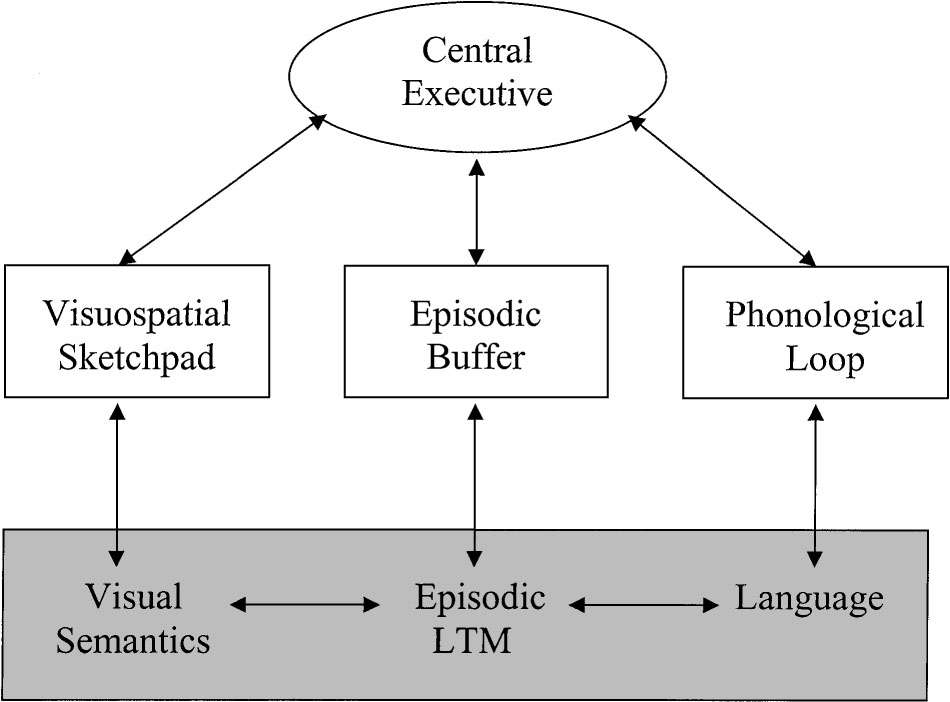
\includegraphics[width=0.5\linewidth]{baddeley-wm}
					\caption[Baddeley and Hitch Working memory model]{Working memory model by Baddeley and Hitch, displaying the 'slave systems' visuo-spatial sketch pad, episodic buffer and phonological loop, controlled by the central executive.}
					\label{fig:baddeley-wm}
				\end{figure}		
				

			We can also consider the multiple resources model by Wickens\cite{wickens2008multiple,wickens2002multiple} which is suited for predicting the workload of an operator performing multiple tasks at one time. The approach is based on four basic assumptions:\\

			1) in the stages of processing dimension, perceptual and cognitive tasks use different resources than response selection and execution;\\
			2) spatial activity uses different resources than verbal or linguistic activity;\\
			3) the modalities dimension, different resources are used for auditory and visual perception\\
			4) visual channels are divided on focal and ambient vision\\
			And the main argument of the theory is ``to the extent that two tasks use different levels along each of the three dimensions, time-sharing will be better'' \cite{wickens2008multiple}. The model provides an account on how different elements of the human information processor, like attention, perception, working memory, response selection and execution interact between each other. This theory is also based on evidence from cognitive neuroscience where we can see that different modalities have different locations in the human brain, like primary auditory cortex is involved with auditory perception[] and the visual perception is processed in the occupational lobe[].\\
				\begin{figure}[h]
					\centering
					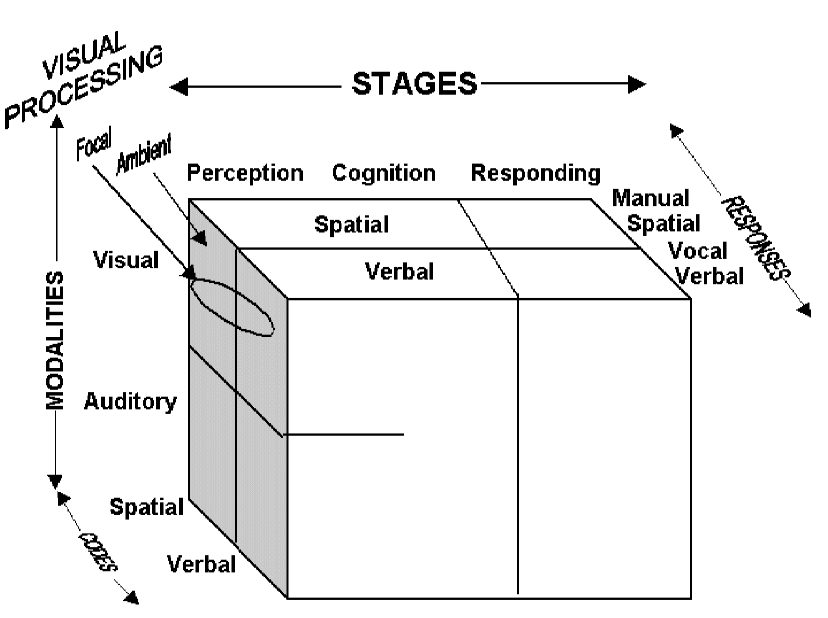
\includegraphics[width=0.7\linewidth]{mrt}
					\caption[Multiple resource theory by Wickens]{Wickens 4-D multiple resources model}
					\label{fig:mrt}
				\end{figure}
			However, mental workload can be influenced by the initial perception of the task at hand or the 'appraisal' of it. Similarly to MW appraisal is complex and multidimensional concept\cite{folkman1986dynamics,peacock1990stress} that is not well defined.
		
			\subsection{Measuring Mental Workload}
			The concept has been explained differently by different authors, and inferences made from various empirical measures which can be divided on primary, secondary, subjective and psychophysiological measures. There are also analytical techniques but we are not concerned with them in this dissertation.
				\subsubsection{Primary and secondary task measures}
				Primary measures rely on operator performance to predict workload. However, a limitation of using primary measures alone is that an operator can spend high amount of effort but this may not be apparent from the performance\cite{wilson2015evaluation}. Consequently, primary task measures should be combined with other workload measures. An example performance measures are task completion time, number of errors, and response time. In our case we will use a combination of all but secondary task measures. Secondary task involves inclusion of a additional simple task to the primary one, which is done concurrently, if the primary task has low or moderate demand and the level of workload cannot be inferred only from the primary measure. It is used to detect when operators performance deteriorates and this is due to workload overload. However, as we are not going to use secondary measures, more explanation will provided for the other types of measurements.
				\subsubsection{Subjective measures}
				Subjective measures use rating scale and are based on operator opinion of their perceived workload during or after completion of task. They are preferred method for WL estimation because they are easy to administer, cheap, and with high face validity. They are classified as uni dimensional and multidimensional. They consist of single subjective scale of workload and multiple scales of types of workload, accordingly. From the unidimensional subjective measures the Cooper-Harper\cite{cooper1969use} is the most popular among ergonomists and cognitive researchers. However, it is designed for the aircraft domain, and therefore a modified cooper-Harper scale\cite{wierwille1983validated} was created for use in other domains. However, as mental workload is influenced by different environmental and personal factors\cite{rouse1993modeling}, therefore the concept of MW should be considered as multidimensional concept, in order to improve diagnosticity. Accordingly, multi-dimensional subjective scales should be used to better understand the aspects of MW. The most used scales are NASA-TLX\cite{nasatlx}, SWAT\cite{reid1988subjective} and Workload profile\cite{tsang1996diagnosticity}. NASA-TLX is based on rigorous laboratory research, and it includes 6 scales (mental, physical, temporal demand, experienced effort, frustration and performance) consisting of 20 intervals each and it is relatively easy to administer. In addition, a single measure of workload can be weighted, although it is not necessarily required because there is high correlation between weighted and unweighed results\cite{byers1988workload}. 
				The SWAT subjective scale is also widely used, however the process of implementation is laborious and more complex than the other subjective scales. The other popular scale is Workload profile(WP)\cite{tsang1996diagnosticity} scale which is basen on the Wickens multiple resources model, and asks questions about each of the four dimensions proposed by the theory. Hence, it is very useful when combined with multiple resource theory interpretation of the results. Finally, Longo et al. \cite{longo2012importance} compared the three measures mentioned above in a web browsing/searching task, and observed correlations in the results of the three measures claiming that they measure the same concept of mental workload.\\
				\subsubsection{Psychophysical measures}
				Psychophysical measures are used to give objective data about mental workload by not relying on subjective scales or performance measures . They can be obtained by recording cardiac activity, electrodermal activity, eye function or imaging the brain. These techniques detect the  change in the arousal from the autonomic nervous system level which can be inferred to as mental workload. However, different psychophysical measures capture different aspects mental workload\cite{cain2007review}, therefore consideration should be put in choosing the most appropriate measure for the given task. \\
				Mean heart rate(HR) and heart rate variability(HRV) are one of the most used techniques to infer arousal because it is relatively cheap and easy to administer. However, HR not always correlates to subjective measures of MW\cite{haapalainen2010psycho} and because of this HRV can be considered as more valid measure. Moreover, the beat to beat interval of the heart can be measured using different statistical approaches\cite{billman2011heart}, like, standard deviation from heart beat intervals. Measurements of eye activity, like blink rate, pupil diameter are also being found to correlate to MW. Furthermore, increase in pupil diameter is correlated to rise in arousal \cite{kahneman1973attention}, and Beatty claimed that it has high sensitivity \cite{beatty1982task} and it can be used to distinguish between data-limited and resource limited processing, which can make it very useful in the HCI field. However, incoming light at the eye can change the pupil diameter, which is a process unrelated to the task, thus influencing the measurements, therefore it is suitable for experiments in controlled environment. \\Finally, a number of brain imaging techniques are used to obtain measurements from the brain activity, including electroencephalography(EEG), functional near-infrared spectroscopy(fNIRS), functional magnetic resonance imaging(fMRI), however these will be discussed later in section "Brain sensing".
		
		 %and yielded similar results, suggesting they measure the same aspects of the web task. The author infers that only one mental workload measure is required. Because mental workload is influenced by a number of factors, and therefore it is multidimensional concept, NASA-TLX is chosen as subjective measure for the experiment.
		
 
		 %Lavie(2005,2010) Load theory says high perceptual load decreases attention to distractions, and low perceptual load increased them. High perceptual load is experienced when, for example, driving fast a car, or playing sports. Furthermore, because it involves a lot of perceptual capacity there is no spare capacity for the attention to perceive distractions. In this case, the task has a low perceptual load because it demands only to a visual stimuli to be percieved and processed rather than with audioty, o

	\section{Emotion processing}
		To begin with, mood and emotion are frequently referred as separate concepts. For example, emotions are thought to last for shorter time like, several minutes, in comparison to moods which can last for a whole day or more. Also, emotions are generally caused by certain events, like winning a game, in contrast to moods where often there is no reason as to why an individual is in certain mood. However, there is no clear distinction between them because moods can cause certain emotions and emotions can cause moods. To solve that problem researchers often use the term ``affect'' to encompass both emotions and moods. Furthermore, we can define positive moods or emotions as positive affect, and negative emotion and moods as negative affect.
		
		There are two major approaches in describing emotions - the categorical\cite{izard2007basic} and the dimensional approach\cite{feldman1998independence}. The first one, categorises several different emotions like, happiness, sadness, anger, fear, and disgust, and often matches the subjective experience of individuals. The second one, the dimensional approach considers emotions to have two distinct dimensions of pleasure-misery (emotional valence) and arousal-sleep.  
		\begin{figure}
			\centering
			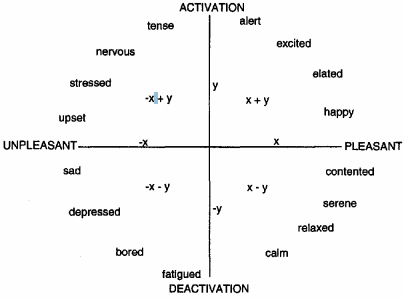
\includegraphics[width=0.7\linewidth]{two-demensional-approach-emotions}
			\caption[Two dimensional approach of emotion]{The two dimensional approach of emotion. The x and y axes represent semantic components: x=pleasant and unpleasant emotions, and y=level of activation. The image is taken from Russell and Feldman ``Independence and bipolarity in the structure of current affect''\cite{feldman1998independence} }
			\label{fig:two-demensional-approach-emotions}
		\end{figure}
		For example, the happy emotion can be pointed to have high positive valence and moderate activation or arousal. In contrast, the emotion of sadness has high negative valence and again moderate arousal. Furthermore, there is a considerable debate on which approach should be adopted by researchers\cite{fox2008emotion}, however we decided to use the dimensional approach because we wanted to have a numerical measure of emotional valence, which than can be compared to the objective data.
		
		Also, emotion processing depends on top-down(appraising a situation based on similar previous knowledge) and bottom-up(processing external stimuli) processes. The first one(top-down) is more cognitive process because it uses attention and memory in order to assign a valence to a given stimuli. The bottom up processing is influenced by external stimuli, so it uses more visual perception. Generally, there are considerable differences between them, and many theorists considers which one of them is more involved with emotion generation. However, there are many ``appraisal theories'' that suggest cognition strongly influences when we experience emotional states and what particular states we experience in a certain moment. For instance, one can appraise a non-threatening situation as threatening and therefore she will experience negative valence. Moreover, many theorists argue that appraisal is both conscious and automatic. Smith and Kirby\cite{smith2009putting} suggested two types of appraisal: one that is based on reasoning(deliberate thinking), and one that is based on activation of memories(automatic processes). The first one is claimed to be slower and more flexible. 
		
		It has been assumed that emotional states influence cognition\cite{blanchette2010influence}, like attention, perception, decision making, and others. Also, what we remember from a situation is strongly affected by what we attended during that time\cite{eriksen1986visual}. In addition, an influential theory by Easterbrook\cite{easterbrook1959effect} suggest the number of attentional cues processed declines as arousal or anxiety increases. It can be interpreted as strong negative valence delivers "tunnel vision", and positive valence produces breadth of attention. For example, a individual in highly stressful situation, like auto mobile incident, will remember only the low amount of details related to the moment of the accident. In contrast, when one is experiencing positive situation, it is likely that she will remember more unrelated details about the event. However, Harmon-Jones et al.\cite{harmon2011toward} argued that the above mentioned theory considering only emotional valence is over simplified and it lacks the addition of \textit{motivational intensity}. Generally, there are two types of motivation: approach and avoidance motivation. According to the authors the approach motivation can be low, for example listening to music, or high, for instance recognizing a attractive subject from the opposite sex. On the other hand, low avoidance motivation can be exposure to unfair situation, and high avoidance motivation can be dealing with life-threatening situation. Harmon-Jones et al.\cite{harmon2011toward} postulated that high motivational intensity leads to narrowing of the attention for both positive and negative experiences because it helps individuals to successfully accomplish tasks. On the contrary, low motivational intensity for both positive and negative experiences leads to attentional broadening because individuals leave spare attentional resources, in order to be able to encounter and react accordingly to a new and maybe more valuable situation.
		
		Russell\cite{russell2003core} proposed a valence model of emotion which states that significant higher activation of the left hemisphere compared to the right was associated with positive emotions, whereas significantly higher activation in the right hemisphere should be associated with negative emotion. Therefore, we can infer whether an affect was positive or negative if we measure the brain activation during an experiment.
		
		Generally, there are two main types of measuring emotion processing: objective and subjective. One subjective measurement technique is the self assessment manikin(SAM)\cite{bradley1994measuring}, which we used because it provides two scales - emotional valence and arousal and. Other widely used measure is the Positive and Negative Affect Schedule(Panas)\cite{watson1988development}. However, it is more complex to use, for example, explain to participants how to use it, and therefore not really suitable for complex cognition experiments. Also, the scales had visual icons that help participants recognise what each point of the scale means. The objective techniques that try to infer emotional valence include psychophysiological measures of galvanic skin response, heart rate, respiration\cite{krumhansl1997exploratory}, and brain activity\cite{Balconi201567}. We decided to combine subjective and objective measure of emotional valence, in order to compare them and later make inferences about. We chose SAM because it is widely accepted, and easy to implement, and brain sensing technique for the objective measure, as we try to prove the left vs right hemisphere hypothesis of Davidson\cite{davidson1992emotion} which is explained below. Next, we will review brain sensing techniques and pick one suitable for this master thesis experiment.
		
		%10. mood congruity
		%11. Dual process model - fast automatic and affective system and slower effortful and more cognitive system
		
	\section{Brain sensing}
	Initially, brain sensing was used in for medical purposes, however in recent years it has been used in other fields, like cognitive psychology, and lately, for Brain-Computer interface(BCI). We review only brain sensing techniques that are suitable for measuring complex cognition and are non-invasive so it can be used in HCI experiment. First of all, the functional magnetic resonance imaging (fMRI) is measuring the haemoglobin oxygenation and deoxygenation in the brain which is referred to as blood oxygen level-dependent contrast(BOLD) signal. It uses a large magnet which causes a strong magnetic field and a short radio-frequency pulse is emitted, in order to detect areas of activation in the brain. Furthermore, MRI has high spatial resolution which detects activation in brain regions with up to 1mm precision and is suitable for distinguishing particular brain regions of activation for the studied task. Also, its temporal resolution has 2-3 seconds delay, as it takes some time for the neural activity to occur and be detected. Typical fMRI studies involve emotion induction\cite{phan2002functional,brattico2011functional} and mental arhytmetic\cite{kawashima2004functional}. However, during experiments participants should stand still and even the slightest movements can cause artefacts and distort the signal. Therefore, this technique is not suitable for HCI evaluations because subjects cannot physically move.
	
	Another widely used brain imaging technique is the EEG which measures electrical changes at the surface of the scalp. It is non-invasive technique, which makes it suitable for cognitive and HCI research. Waveforms with different bands are calculated from the electrical signal that can later be analysed. The strength of EEG is its temporal resolution as it can detect changes in brain activity with accuracy of a few milliseconds. However, it is highly susceptible to motion artefacts, and even the slightest movement of fingers can cause deformation of the signal. Consequently, it is not suitable for web interface evaluations because when users type on the keyboard or use the mouse will cause considerable distortions of the brain signal. 
	
	A more recent brain imaging technique is the functional near infrared spectroscopy (fNIRS) which unlike EEG is an optical-imaging modality. Furthermore, fNIRS can detect cerebral hemodynamics by calculating the oxygenated haemoglobin(Hbo) and deoxygenated haemoglobin(Hbr). It uses infrared light which is emitted to the participants skull using emitter-detector pairs consisting of infrared LED emitter, and infrared sensors. They usually operate with two or more wavelengths (650-1000nm)\cite{scholkmann2014review}. Furthermore, because Hbo and Hbr have different light absorption coefficients and the infrared sensors can detect the reflected light from them, the concentration of Hbo and Hbr is calculated using modified Beer-Lamberts law\cite{delpy1988estimation}. The fNIRS has low temporal resolution with a 2-8 sec delay\cite{huppert2006temporal,solovey2009using} depending on the task. However, it has good spatial resolution and can detect signals 1cm inside the cortex depending on the emitter-detector configuration, and has shown good correlation with the fMRI data\cite{cui2011quantitative} for cognitive tasks.  Another advantage is that it provides a continuous data and different periods of the task can be defined and later analysed. In addition, fNIRS devices are becoming more and more portable, have high spatial resolution, and most importantly they have low sensitivity to motion artefacts which makes it particularly suitable for HCI studies\cite{maior2015examining,solovey2009using}. Hence, we decided to use fNIRS because of its applicability for usability experiments. For more comprehensive review of the fNIRS brain imaging instrumentation and methodology Scholkmann et al\cite{scholkmann2014review} article provides detailed information.
	Next, relevant studies that try to infer mental workload and emotional valence using fNIRS will be reviewed in the subsections below.
		\subsection{PFC, cognition and emotional processing}
		Generally, the prefrontal cortex(PFC) has been associated with higher cognitive functions by studies examining brain damaged individuals\cite{shallice1988neuropsychology,smith1997working}. Also, experiments on healthy subjects using the n-back task\cite{braver1997parametric} have supported this claim. More specifically, activation was observed in the dorsolateral prefrontal cortex (BA 9/46), inferior frontal (BA 6/44) and parietal (BA 7/44) when the task demanded more working memory resources. However, it is difficult to point which brain region is involved with which processes because one brain area is usually involved in multiple cognitive tasks\cite{brown2012common}. Moreover, Yarkoni\cite{yarkoni2011large} supported that claim by reviewing 3489 studies, which considered areas of human brain. Interestingly, activation in the same brain regions (dorsolateral prefrontal cortex, anterior insula and anterior cingulate cortex) was observed in one fifth of the studies. He used a machine learning algorithm and classified different studies into ones that assessed working memory, emotion and pain. It also, can be seen from the graphs that both working memory and emotion processing studies evoked activation in the PFC. Furthermore, individual differences in brain structure exist, especially in the PFC area\cite{thompson2001genetic}. In addition, gender differences in the brain structure are also observed\cite{cosgrove2007evolving}. 
		
		There are also evidence that the PFC is involved with emotion processing and emotion regulation\cite{davidson2002anxiety,damasio1996somatic,balconi2012detection}. More specifically, the ventromedial prefrontal cortex is suggested to be involved in the representation of positive and negative emotional states, and the dorsolateral prefrontal cortex in the representation of the goal states towards these affective states are directed. Also, it is suggested that amygdala processes threat stimuli and processes negative affect of fear\cite{davidson2002anxiety}. Furthermore, the orbitofrontal cortex in the PFC has been linked to reward processing and reinforcement learning\cite{rolls2000orbitofrontal}, therefore playing a role in the assignment in emotional valence and intrinsic motivation.
		
		Davidson proposed the ``valence asymmetry hypothesis'' which states that positive affect which is linked to approach motivation is experienced when the left frontal cortical region has higher activation than the right. In contrast, negative affect which is linked to avoidance motivation is experienced when more activation is observed in the right frontal cortical region compared to the left. Also, the valence model of emotions by Russell\cite{russell2003core} supports this hypothesis. Consequently, we are interested in using fNIRS in order to measure the activations in left and right frontal hemispheres and interpret the results using the \textit{valence asymmetry hypothesis}. We will review more relative studies that used fNIRS to investigate the relationship between left and right hemispheres in the ``fNIRS and Emotional Valence'' subsection below. 
		
		\subsection{Fnirs and Mental Workload}
			In this subsection we review studies that has used fNIRS for measuring the mental workload in cognitive tasks. According to our knowledge there is only one study using fNIRS for evaluation of visualisation interfaces, and more specifically comparing bar graphs and pie charts. They could not find statistically significant results between the two from the hemodynamics data
			Highlight studies involving mental workload.
			More specifically,
			there is a positive correlation between the increase of oxygenated blood and the
			increase in cognitive WL- 
			-limitations
			has low temporal resolution
		\subsection{fNIRS and Emotional Valence}
			It is still not proven that activation in the left hemisphere is responsible for the processing of positive emotion.
			gender differences, 
			left-right handedness
			1. Emotional induction - when pictures or videos or other method is used to trigger certain kind of emotion
			Emotional regulation
			- apprisal
			- reapprisal - kogato si spomnime i preocenim dadena emociq (cognitively reexamine the meaning of emotional events)
			- anticipation of expected outcomes 
			- In this study we have combined "hot" emotional control  with cold control of attention and memory, as suggested by Kevin N. Ochsner and James Gross \cite{the-cognitive-control-of-emotion}
			-Richard Davidson first a comprehensive research in the topic cortical assymetry
	\section{Summary}
		Because not many researchers[] do not take in consideration the emotional state(positive or negative) which can be related to aproach and avoid motivation during task execution, and how it influences the performance of the operator and perceived workload, we have combined multidimensional subjective scale (NASA-TLX) with emotional valence scale (SAM). By combining the these subjective measures and comparing them the objective measure of mean Hbo from the fNIRS device we expect to gain better understanding of the operator performance during the web form filling task.
		Arrousal should correlate with skin conductance.
		We are aiming to reduce to imposed load by the task by minimizing the visual search(condition3) and aiding the episodical memory by placing a description in the beginning of the form.
\chapter{User study}
	\section{Hypothesis and expectations}
	Based on the literature review we state the following hypothesis:\\
	1) There is significant statistical difference between the three web forms\\
	2) Subjective data from NASA-TLX correlates to objective data from the fNIRS\\
	3) The difference in left and right hemisphere activations correlate to subjective SAM scale of emotional valence\\	
	\section{Method}
	Describe why I have used the following methods, including the perceived benefits of your approach\cite{preferences-study}.
		\subsection{Participants}
		\subsection{Apparatus}
			\subsubsection{Laptop computer}
			The experiment was executed on 15" laptop, HP probook 450 with screen resolution 1366x768. The participant was presented with a screen with links to the three different videos and web forms. They were instructed by the researcher to manually start certain condition or video. 
			\subsubsection{fNIRS}
			Picture of fNIRS\\
			730nm and 850nm wavelengths will be collected for each voxel, eliminating the ambient light. . However, if the data acquisition computer does not have enough bandwidth,
			one or more of the quadrants can be disabled to maintain 2Hz sampling rate. 
			\subsubsection{Empatica}
			Picture of Empatica E3\\
			Before attaching the Epatica E3 the skin was treated with alcohol for better conductivity. maybe remove
        \subsection{Materials}
			\subsubsection{NASA TLX}
			\subsubsection{SAM}
			\subsubsection{Web forms}
			\subsubsection{Video capture}
		\subsection{Design}
		The study used repeated measures within subjects design. The three variations of videos and the web forms were counterbalanced, in order to avoid learning effects from the order of presentation of the video clips.
		Performance measure - characters written in the description field
		\subsection{Procedure}
		First, participants were asked to read and sign information sheet and consent forms. Second, the Empatica E3 and fNIRS devices were cleaned then equipped and started. Third, participants were briefed about the procedure of the experiment, and it was explained how to fill the subjective scales. Also, because of ethical considerations that the participant should not enter personal data in the web form, a fake personal credentials were provided, that she should fill in the web forms. Fourth, after the video capture, fnirs and empatica devices started recording data, participants were asked to open one of the three videos, depending on the counterbalancing table. After the video was finished, participants fill SAM subjective scale. Fifth, there was approximately 2 minute waiting period so that participant's memory is not fresh before she was asked to open one of the three web forms, again depending on the order from the counterbalancing table. Finally, after participant has completed the web form, the SAM and then the NASA-TLX scales are given to be completed, accordingly. This process was repeated three times, following the within subjects experimental design.
		Before each experiment, the clocks between the two computers (the one that was obtaining the information and one that participant worked on) were synchronized. Also, timestamps using the Cobi Studio software manual markers were created in the beginning and end of each condition and video. 
		\subsection{Data Analysis}
		The fNIRS data was analyzed with NIRS-SPM\cite{ye2009nirs}		
			\subsubsection{Signal acquisition}
			What is the task - it is not mental aritmetic, or mental imagery, it is complex web form filling task.
			\subsubsection{Preprocessing}
			Instrument noise was reduced by placing a hat over the fNIRS headband, in order to block external light.
			First, low-pass filter with cut off frequencies of 0.1 Hz, was used in order to remove physiological noise, like heartbeat and blood flow movement that is not associated with brain activity or Mayer waves.
			Then, the NIRS signal was processed with modified Beer-Lambert law\cite{cope1988system}, in order to calculate oxygenated, and deoxygenated hemoglobin values.
			Finally, to remove motion artefacts, the correlation based signal improvement(CBSI)\cite{cui2010functional} method was applied to the data.
			\subsubsection{Feature Extraction/selection}
			After data preprocessing we should choose what features we will use to evaluate our data - mean values of oxy-Hb, mean values of oxy-Hb for all channels, skewness, variance
	\section{Results}
		\subsection{Mental Workload}
			\subsubsection{fNIRS data}	
			A one-way repeated measures ANOVA was conducted to determine whether there was a statistically significant difference in mean Hbo values between the three web forms. The assumption of sphericity was met, as assessed by Mauchly's test of sphericity, $X^{2}(2) = 0.195, p = 0.907$. There was no significant statistical difference in the mean Hbo between the 3 web forms  $F(2,20)=3.400, p<.054,$ partial $\eta^{2}=.254$ with mean Hbo decreasing from 0.2377 (SD = 1.19) in index3 to -0.1166 (SD = 0.82) and -0.117 (SD = 1) for index2 and index1 respectfully.
			After conducting t-tests between index1 and index3 there was found a marginal statistical difference p=0.054. Which means that the measured Hbo between the two versions has a 94.6\% statistical chance that the difference is not caused by random sampling error. However, we fail to reject the first null hypothesis. This means that we could not find a statistically significant interaction, however we were very close to statistical significance, as p=0.054 and we can assume we have marginal statistical significance.
				\begin{figure}[h]
					\centering
					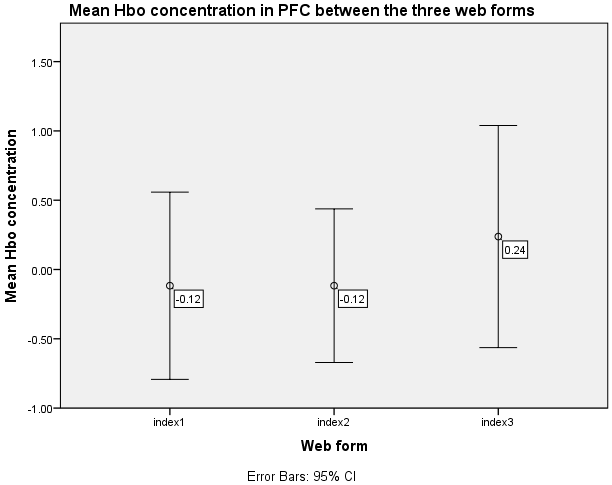
\includegraphics[width=0.7\linewidth]{mean-hbo-index123}
					\caption[Mean oxygenated hemoglobin between the three web forms]{}
					\label{fig:mean-hbo-index123}
				\end{figure}	
			No statistical significance was found when comparing the means of Hbr between the three conditions $F(2,20)=2.044, p<.156,$ partial $\eta^{2}=.170$ where index2 had the highest Hbr mean 0.05 (SD = 0.85), index1 with -0.07 (SD = 0.96) and index3 with the lowest Hbr mean -0.36 (SD = 1.43). Also, a repeated measures ANOVA test was conducted to elicit significant statistical differences between mean Hbt between the three web forms, however no statistical significance was found $F(2,20)=0.685, p<.516,$ partial $\eta^{2}=.064$ where index2 had the highest Hbt mean -0.08 (SD = 0.49), index3 with -0.13 (SD = 0.58) and index1 with the lowest mean Hbt -0.19 (SD = 0.49). The results indicate that Hbo was more responsive for this experiment and gave us higher significance between condition compared to Hbr and Hbt.
			\subsubsection{NASA-TLX}
				There was no statistical significance between each of the NASA-TLX scales, including the total$F(2,38)=0.743, p<.482,$ partial $\eta^{2}=.038$ score as assessed by one way repeated measures ANOVA. Which means statistically we have 51.8\% chance of the results of the total NASA-TLX score to be caused by random sampling error. Also, perceived mean mental demand was lowest for index1 9.15 (SD = 4.94), index2 had slightly higher mean 9.40 (SD = 4.68) and index3 has the highest scores 10.8 (SD = 5.38). Also, mental demand had a strong positive correlation with total tlx for the 3 conditions $r(18)=0.652, p=0.002$, $r(18)=0.738, p<0.001$, and $r(18)=0.741, p<0.001$ for index1, index2 and index3 respectfully. Which supports the validity of NASA-TLX measurements. The total calculated value for the NASA-TLX was highest for index3 7.07 (SD = 3.22) decreasing to 6.92 (SD = 2.95) for index1 and 6.47 (SD = 3.11) for index2. This means that index3 requires slightly more attentional resources to complete the task compared to index1 and index2.
				There was a moderate positive correlation between mental demand scales and task completion times between the three conditions  $r(18)=0.487, p=0.030,  r(18)=0.484, p=0.030,  r(18)=0.638, p=0.002$. This means the more participants perceived higher workload the more their performance dropped as it took them more time to complete the task.
				\begin{table}[h]
					\centering
					\caption{NASA-TLX mean scores}
					\label{my-label}
					\begin{tabular}{l|ccc}
						& Index1           & Index2           & Index3           \\[0.12cm]   \hline
						Mental demand   & 9.15 (SD = 4.94) & 9.40 (SD = 4.68) & 10.8 (SD = 5.38) \\
						Physical demand & 4.05 (SD = 4.08) & 2.90 (SD = 3.21) & 3.90 (SD = 3.65) \\
						Temporal demand & 7.40 (SD = 4.49)  & 7.65 (SD = 5.79) & 6.55 (SD = 4.91) \\
						Performance     & 6.65 (SD = 3.79) & 5.60 (SD = 3.62)  & 6.20 (SD = 3.86)  \\
						Effort          & 8.15 (SD = 4.58) & 7.35 (SD = 4.68) & 8.20 (SD = 5.30)   \\
						Frustration     & 6.10 (SD = 5.11)  & 6.00 (SD = 3.66)  & 6.75 (SD = 5.22) \\\hline
						Total 			& 6.92 (SD = 2.95) & 6.47 (SD = 3.11) & 7.07 (SD = 3.22)
					\end{tabular}
				\end{table}
	
			\subsubsection{SAM - arousal scale}
			The perceived arousal was lowest for index1 2.8 (SD = 0.95) increasing to 2.95 (SD = 1.05) for index2 and to 3.15 (SD = 1.18) for index3 respectfully. No statistical significance was found when comparing the means between the three conditions $F(2,38)=2.462, p<0.099$ partial $\eta^{2}=.115$ using one way repeated measures ANOVA. However, after running post hoc test without adjustments(LSD) a statistically significant difference was found between index1 and index3 $p=0.049$.
			Also, the time to complete index1 and index2 positively correlated to perceived arousal for index 1 and index2:$r(18)=0.551, p=0.012$ and $r(18)=0.473, p=0.035$. However time to complete index3 does not correlate to perceived arousal of index3 $r(18)=0.269, p=0.252$
			
		\subsection{Emotional Valence}
			\subsubsection{fNIRS differences}
			WEB FORMS\\			
				\begin{figure}[h]
					\centering
					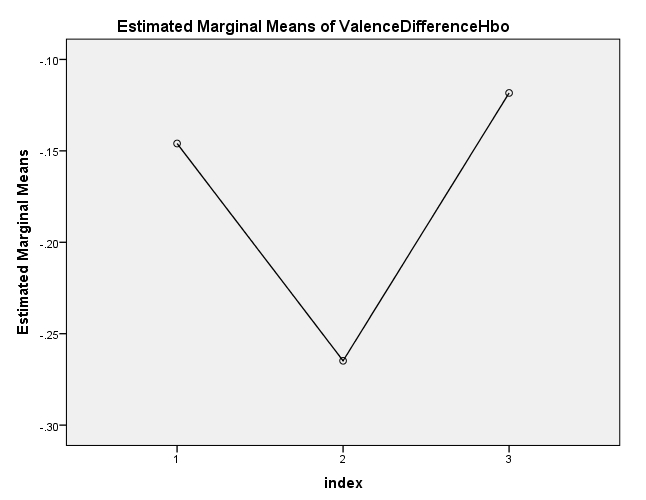
\includegraphics[width=0.7\linewidth]{hbo-valence-differences-index123}
					\caption{}
					\label{fig:hbo-valence-differences-index123}
				\end{figure}
				The fnirs Hbo valence differences was highest for index3 -0.12 (SD = 1.25) decreasing to -0.15 (SD = 1.31) for index1 and the lowest value was for  index2 -0.26 (SD = 1.13).
				The Hbr valence differences were highest for index2 0.34 (SD = 1.18) decreasing to 0.18 (SD = 1.39) for index3 and to 0.10 (SD = 1.68) for index1.
				The Hbt mean valence difference values for index1 were lower -0.45 (SD = 0.79) compared to index2 0.06 (SD = 0.56) and index3 0.05 (SD = 0.87) respectfully. There was no statistical significance as assessed by one way repeated measures ANOVA between the three conditions for Hbo valence differences: $F(2,20)=0.392, p<0.681,$ partial $\eta^{2}=.038$ , Hbr valence differences: $F(2,20)=0.418, p<0.664,$ partial $\eta^{2}=.040$ and Hbt valence differences: $F(2,20)=0.302, p<0.743,$ partial $\eta^{2}=.029$. Also, there was strong positive correlation between temporal NASA-TLX scale of index1 and the Hbo valence differences of index1 $r(9)=0.766, p=0.006$, however, there was no correlation found between index2: $r(9)=0.581, p=0.061$ and index3: $r(9)=0.218, p=0.519$.\\
			VIDEOS\\
				The mean Hbo valence difference for video3 was the highest with 0.17 (SD= 0.25) compared to video1 with -0.01 (SD = 1.32) and video2 with -0.8 (SD = 1.20). In contrast, mean Hbr valence difference values for video3 were the lowest with -0.25 (SD = 0.47) compared to video1 0.30 (SD = 1.20) and video2 0.32 (SD = 0.89). For the mean Hbt valence difference values video1 was the highest with 0.18 (SD = 0.71) decreasing to 0.07 (SD = 0.64) for video3 and to -0.06 (SD = 0.35) for video2.\\
				A one-way repeated measures ANOVA was conducted to determine whether there was a statistically significant difference in Hbo, Hbr and Hbt valence differences between the three videos. There was no significant statistical difference in the mean Hbo valence difference between the 3 videos $F(2,20)=0.051, p<0.951,$ partial $\eta^{2}=.005$, the mean Hbr valence difference: $F(2,20)=0.062, p<0.940,$ partial $\eta^{2}=.006$ and the mean Hbt valence difference: $F(2,20)=0.522, p<0.601,$ partial $\eta^{2}=.050$.
				There was no correlation found between Hbo valence differences and SAM emotional valence subjective scale for the three videos $r(9)=-0.490, p=0.126$; $r(9)=0.095, p=0.781$; $r(9)=0.496, p=0.121$. 
			\subsubsection{SAM emotional valence}
			WEB FORMS\\
				The perceived mean emotional valence for index1 was the lowest with 
				3.1 (SD = 0.97) increasing to 3.4 (SD = 0.99) for index2 and to 3.7 (SD = 0.98) for index3.
				A one-way repeated measures ANOVA was conducted to determine whether there was a statistically significant difference in SAM emotional valence scale values between the three web forms. The assumption of sphericity was met, as assessed by Mauchly's test of sphericity, $X^{2}(2) = 0.446, p = 0.800$. There was no significant statistical difference in the SAM emotional valence scale between the 3 web forms  $F(2,38)=2.803, p<.073,$ partial $\eta^{2}=.129$ with mean SAM emotional valence increasing from 3.1$\pm$0.97 in index1 to 3.4$\pm$0.99 and 3.7$\pm$0.98 for index2 and index3 respectfully.\\
			VIDEOS\\
				The perceived mean emotional valence for video3 was the highest with 3.1 (SD = 1.07) decreasing to 2.9 (SD = 1.33) for video1, and 2.7 (SD = 0.98) for video3. There was no statistical significance as assessed by one way repeated measures ANOVA between the three videos for SAM emotional valence: $F(2,38)=0.792, p<0.460,$ partial $\eta^{2}=.040$.
		\subsection{User performance and preferences}
		The mean time to complete index2 was the lowest 214.88 (SD = 63.81) increasing to 228.79 (SD = 65.19) for index1 and to 231.60 (SD = 83.33) for index3. However, users mostly preferred index3 and index1 with 10 and 9 votes respectively compared to index2 which was preferred by 3 participants.  
		A one-way repeated measures ANOVA was conducted to determine whether there was a statistically significant difference in time to complete between the three web forms. There was no significant statistical difference in time to complete between the 3 web forms  $F(2,38)=0.556, p<.578,$ partial $\eta^{2}=.028$. 
		Also, the time to complete index2 and index3 had a strong positive correlation with perceived effort(NASA-TLX) for index2 and index3: $r(18)=0.702, p=0.016,$ and $r(18)=0.634, p=0.036,$. However, time to complete index1 does not correlate to perceived effort of index1 $r(18)=0.216, p=0.524$

\chapter{Discussion}
	What was the purpose of the study, and then interpretation of the results
	
	fNIRS needs approximately 20 participants, in order to reach statistical significance, however that is four times more than the suggested 5 users tests by Virzi\cite{virzi1992refining}.
	\section{Implications for Design}
	\section{Disadvantages of the study}
		The study tries to simulate real conditions, and therefore lacks ecological validity because users wait approximately 2 minutes after they have watched the video to start filling the web form. This way they still hold some of the information in their working memory and the study is trying to simulate long term memory recall.
	\section{Future work}
	\section{Conclusion}
		In summary, the mental workload is lower for this....

	\section*{Graphs:}
		\begin{figure}[h]
			\centering
			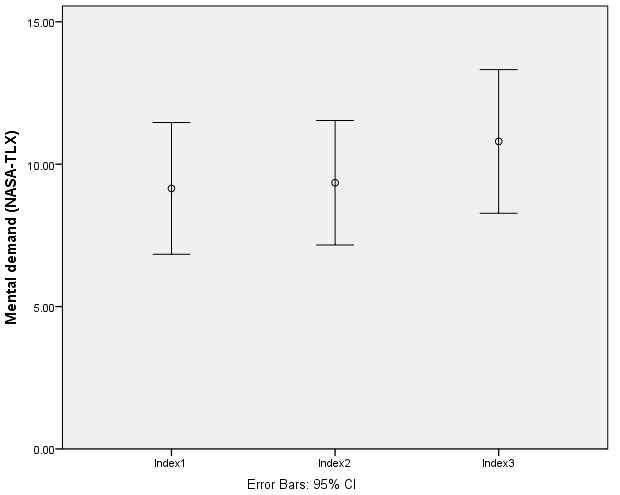
\includegraphics[width=0.6\linewidth]{mental-demand-graph}
			\caption{}
			\label{fig:mental-demand-graph}
		\end{figure}

	\addcontentsline{toc}{chapter}{References}
	\bibliographystyle{plain}
	\bibliography{exmplref}
	\addcontentsline{toc}{chapter}{Appendix}
\chapter*{Appendix}
\end{document}